 \documentclass[a4paper,10pt]{article}
\input{/Users/WannaGetHigh/workspace/latex/macros.tex}

\title{TP2 : Codage d'un contour}
\author{Benjamin \bsc{Van Ryseghem} Fran�ois \bsc{Lepan}}

\begin{document}
\maketitle

\section{Codage d'un contour}

\subsection{Cont}
Les points du contour sont stock� dans la variable sous forme d'une liste de nombre complexe.

\subsection{En ne conservant qu'un point sur 4, puis un point sur 8, constituer deux autres contours approchant la forme circulaire et les afficher respectivement en bleu et en vert dans la m�me fen�tre}

Voici le code correspondant:

\begin{Verbatim}
nom1 = "cercle-80.txt";
cont1 = rdfChargeFichierContour (nom1);

cont2 = cont1(1:4:$);
cont3 = cont1(1:8:$);
rdfAfficheContour(cont1, 2, "r");
rdfAfficheContour(cont2, 2, "g");
rdfAfficheContour(cont3, 2, "b");
\end{Verbatim}

\section{Descripteur de Fourier}

\subsection{Pourquoi la fonction rdfDescFourier �limine t'elle parfois un point de la liste des points du contour?}
Pour plus de performance dans le calcule des descripteurs de Fourier

\subsection{V�rifier que les descripteurs de Fourier permettent de reconstituer le contour initial}
Voici le code correspondant:
\begin{Verbatim}
descFour = rdfDescFourier(cont);
rdfAfficheContour (rdfInverseDescFourier(descFour), 1, "k");
\end{Verbatim}

\subsection{Quel est l'indice de tableau correspondant au descripteur Z0 ?}
Il se situe � la moiti� de la taille du tableau.

\subsection{Expliquer l'utilit� de la fonction rdfValeurDescFourier}
Cette fonction sert � afficher la valeur d'un point de la liste des descripteurs de Fourier 
 
 \subsection{A quoi correspond le descripteur de Fourier $Z_0$ d'une forme d�crite par son contour?}
 C'est le barycentre de la forme.
 
 On observe que si on met une grande valeur les courbes on tendance a se rapprocher du centre. 
 C'est un peut comme si on augmentait la gravit� au centre de la forme. 
 
\begin{Verbatim}
descFour = rdfDescFourier(cont)
descFour((size(descFour,1)/2)) = VALUE;
\end{Verbatim}

\section{Filtrage des descripteurs de Fourier}

Voici la fonction rdfAnnuleDescFourier:

\begin{Verbatim}
function vector = rdfAnnuleDescFourier(desc,ratio)
    size = size(desc,1);
    
    if ratio == 1 then
        vector = desc
    else 
        if ratio == 0 then
            vector = zeros(1,size)
        else
            index = int(ratio*size)
            
            if ratio <= 0.5 then
                s = size/2;
                s1 = size/2 + 1;
                s2 = size/2 + index;
                s3 = size - size/2 - index - 1;
                vector = [ zeros(1,s)  desc(s1:s2)'  zeros(1,s3)]'
            else
                s = index - size/2;
                s1 = size - index;
                s2 = size/2 + 1;
                vector = [ desc(1:s)' zeros(1,s1) desc(s2:$)' ]'
            end
         end
    end
endfunction
\end{Verbatim}

Lorsque nous r�duisons le ratio il se trouve que en effet la forme se simplifie (faire figure 1).
\section{R�duction d'une cha�ne de contour}

Voici le code que nous sons mis pour rdfAlgorithmeCorde:
\begin{Verbatim}
    if real (debut) == real (fin)  then
        d = abs(real(cont) - real(debut))
    else	
        a = (imag(fin) - imag(debut))/(real(fin) - real(debut))
        b = imag(fin) - a * real(fin)
        		
        if a == 0 then
            d = abs(imag(cont) - b)
        else
            d = abs(a*real(cont) - imag(cont) + b) ./ (sqrt(1+a^2))
        end
    end
\end{Verbatim}

Et on observe bien que si on augmente dmax on r�duit bien le contour (voir figure 2)

\section{Comparaison des deux approches}

Apr�s avoir fait quelques tests nous nous sommes rendu compte que:
Pour des formes connexes (triangles, carres, cercles) l'algorithme des cordes est mieux car beaucoup plus rapide que celui des descripteur de Fourier. Sinon dans les deux cas le travail est bien fait. (voir figure 3) \\
\\
Mais pour ce qui est des formes non connexes ( patato�de) l'algorithme de Fourier est bien plus pr�cis. On observe sur la figure suivante les deux algorithmes et on voit bien que l'algolrithme des cordes fait des segment qui sont en dehors de la figure. (voir figure 4) \\
\\
En conclusion je dirai que l'algorithme des cordes n'est pas aussi efficace pour faire de la reconnaissance de formes complexe comme un visage ou une patate que l'algorithme de Fourier. Par contre il est beaucoup plus rapide pour des formes g�om�triques simples comme un triangle ou un carr�.

\begin{figure}[ht]
\begin{center}
     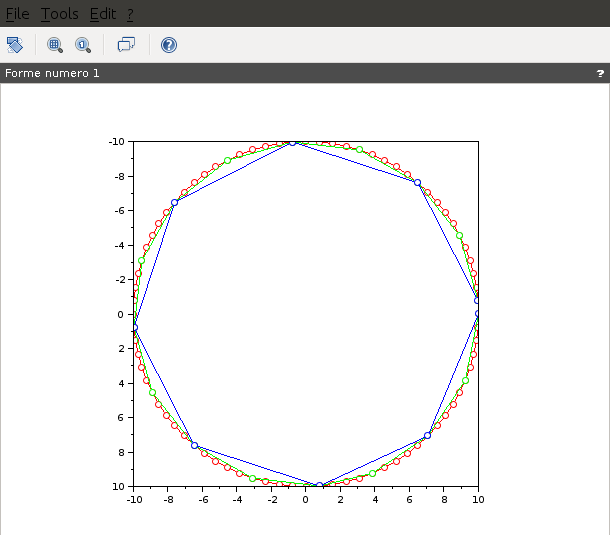
\includegraphics[width=10cm]{reduc_chaine_cont.png}
\end{center}
    \caption{rouge: contours initial \_\_ vert:  Cordes avec dmax=0.5 \_\_ bleu  Cordes avec dmax=1}
\end{figure}

\begin{figure}[ht]
\begin{center}
     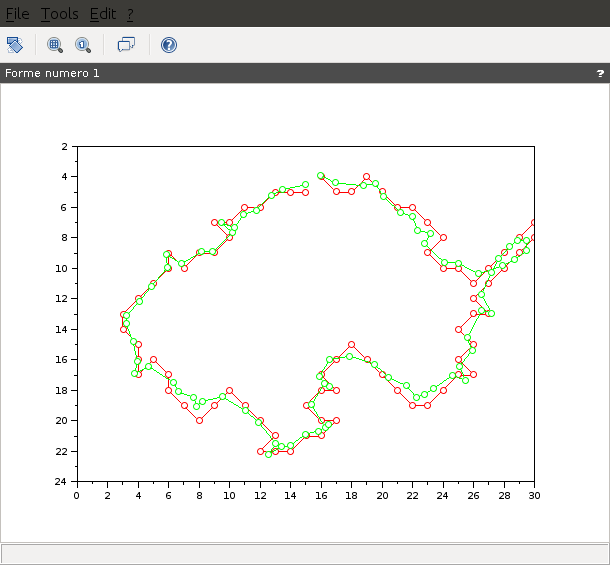
\includegraphics[width=10cm]{cmp_fourier_normale.png}
\end{center}
    \caption{rouge: contours initial \_\_ vert: Fourier avec ratio=0.6}
\end{figure}


\begin{figure}[ht]
\begin{center}
     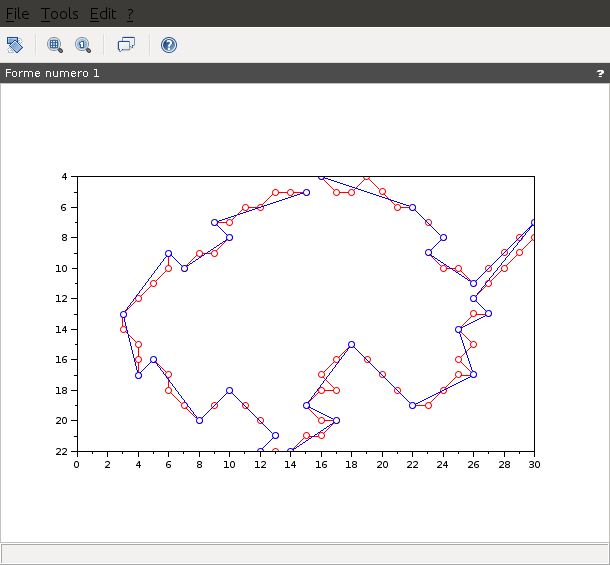
\includegraphics[width=10cm]{cmp_cordes_normale.png}
\end{center}
    \caption{rouge: contours initial \_\_ bleu: Cordes avec dmax=1}
\end{figure}

\end{document}